\documentclass[10pt,letterpaper]{article}

\usepackage[utf8]{inputenc}
\usepackage[T1]{fontenc}
\usepackage{lmodern}
\usepackage[margin=0.45in,top=0.40in,bottom=0.40in]{geometry}
\usepackage{amsmath,amssymb,bm}
\usepackage{graphicx}
\usepackage{booktabs}
\usepackage{tabularx}
\usepackage{xcolor}
\usepackage{hyperref}
\usepackage[expansion=false]{microtype}
\usepackage{tcolorbox}
\usepackage{titlesec}
\usepackage{enumitem}

\graphicspath{{../figures/}{../../docs/engineering_reports/figures/}}

\definecolor{planetblue}{RGB}{0, 100, 180}
\definecolor{planetteal}{RGB}{0, 175, 170}
\definecolor{darkgray}{RGB}{35, 42, 54}
\definecolor{lightbg}{RGB}{246, 252, 254}
\definecolor{bordergray}{RGB}{210, 235, 245}

\hypersetup{
    colorlinks=true,
    linkcolor=planetblue,
    urlcolor=planetteal,
    citecolor=planetblue
}

\pagestyle{empty}

\titleformat{\section}{\large\bfseries\color{planetblue}}{}{0em}{}[\vspace{-0.4em}\rule{\linewidth}{0.8pt}\vspace{-0.3em}]

\tcbset{
    sharp corners,
    boxrule=0.8pt,
    colframe=planetblue,
    colback=lightbg,
    left=6pt,right=6pt,top=5pt,bottom=5pt
}

\begin{document}

% HEADER BOX
\begin{tcolorbox}[colframe=planetblue,colback=planetblue,coltext=white,boxrule=0pt,top=6pt,bottom=6pt]
\begin{minipage}[c]{0.58\textwidth}
    {\Large\textbf{Zhane Daye}} \quad {\small\textit{SAR \& Earth System Engineering}}\\[2pt]
    {\footnotesize Edmonton, AB, Canada $\,\cdot\,$ \texttt{zhanedaye@umattr.ca} $\,\cdot\,$ \href{https://www.linkedin.com/in/zhane-umattr}{linkedin.com/in/zhane-umattr}}
\end{minipage}
\hfill
\begin{minipage}[c]{0.40\textwidth}
    \raggedleft
    {\large\textbf{TARGET: PLANET LABS}}\\[1pt]
    {\footnotesize\textbf{Role:} Senior Frontend / 3D WebGL Geospatial Software Engineer}\\[1pt]
    {\scriptsize Planetary Scale Multi-Resolution Imagery Streaming}
\end{minipage}
\end{tcolorbox}

\vspace{-4pt}

% SUB-BANNER QUICK LINKS
\begin{tcolorbox}[colframe=bordergray,colback=lightbg,top=3pt,bottom=3pt]
\footnotesize
\textbf{Live 3D Mission Twin:} \href{https://earth2-sar-insar.vercel.app#preset=clean_globe&stage=v3}{\texttt{earth2-sar-insar.vercel.app\#preset=clean\_globe}} $\,\vert\,$ 
\textbf{Report (PDF):} \href{https://earth2-sar-insar.vercel.app/reports/EARTH2_X_BAND_SAR_INSAR_ENGINEERING_REPORT.pdf}{\texttt{SAR\_ENGINEERING\_REPORT.pdf}} $\,\vert\,$ 
\textbf{GitHub v1.0.0:} \href{https://github.com/zrt219/earth2studio/releases/tag/v1.0.0-mission-twin}{\texttt{v1.0.0-mission-twin}}
\end{tcolorbox}

\vspace{-4pt}

% TWO-COLUMN CORE CONTENT
\noindent
\begin{minipage}[t]{0.51\textwidth}
    \section*{The Operational Bottleneck}
    \footnotesize
    Planet captures daily global imagery across hundreds of satellites. Delivering petabytes of multi-resolution rasters (PlanetScope, SkySat, Pelican) to web browsers presents critical client-side bottlenecks:
    \begin{enumerate}[leftmargin=12pt,topsep=1pt,itemsep=1pt,parsep=0pt]
        \item \textbf{GPU VRAM Overload \& Browser Crashes:} Eager texture loading for high-resolution planetary octants exhausts browser WebGL contexts ($> 1.2\text{ GiB}$), triggering crashes on mobile and low-power devices.
        \item \textbf{Garbage Collection Frame Stutter:} Allocating dynamic object arrays inside high-frequency animation loops causes recurrent frame-time spikes, dropping framerates well below $60\text{ FPS}$.
    \end{enumerate}

    \section*{The Engineering Solution}
    \footnotesize
    I engineered a zero-dependency, production-grade \textbf{3D WebGL Digital Twin} that streams 16K global and 131K Sentinel-2 regional LOD tiles with ultra-low resource consumption:
    \begin{itemize}[leftmargin=12pt,topsep=1pt,itemsep=1pt,parsep=0pt]
        \item \textbf{80.8\% GPU VRAM Reduction:} Slashed startup memory from $1,290\text{ MB}$ down to \textbf{248 MB} via distance/frustum-gated lazy octants, off-thread \texttt{ImageBitmapLoader}, and LRU texture caching.
        \item \textbf{Zero-Allocation Particle Buffers:} Built typed array particle pools with \texttt{DynamicDrawUsage} for atmospheric wind streamlines and orbits, eliminating runtime GC allocations and locking \textbf{60 FPS}.
        \item \textbf{Full OGC STAC v1.0.0 Integration:} Native client-side parsing of STAC tasking orders, asset metadata, and spatial footprints.
        \item \textbf{Comprehensive UX Suite:} Real-time city search, keyboard shortcuts modal, telemetry badge, and URL hash deep-linking.
    \end{itemize}

    \section*{Verified Benchmark Record}
    \footnotesize
    \begin{tabularx}{\linewidth}{X r r}
        \toprule
        \textbf{Performance Metric} & \textbf{Standard Three.js} & \textbf{Engineered Twin} \\
        \midrule
        Startup GPU VRAM & 1,290 MB & \textbf{248 MB ($-80.8\%$)} \\
        Desktop Render Framerate & 34 FPS & \textbf{60 FPS Locked} \\
        Mobile Render Framerate & 22 FPS (crashes) & \textbf{60 FPS Fluid} \\
        Global Texture Streaming & Single 4K texture & \textbf{16K Octants + 131K LOD} \\
        WebGL Context Restorations & Frequent lost context & \textbf{0 Crashes (CDP verified)} \\
        E2E Automated Verification & Manual testing & \textbf{105 WebGL E2E Tests} \\
        \bottomrule
    \end{tabularx}
\end{minipage}
\hfill
\begin{minipage}[t]{0.46\textwidth}
    \section*{Visual Mission Twin Artifact}
    \centering
    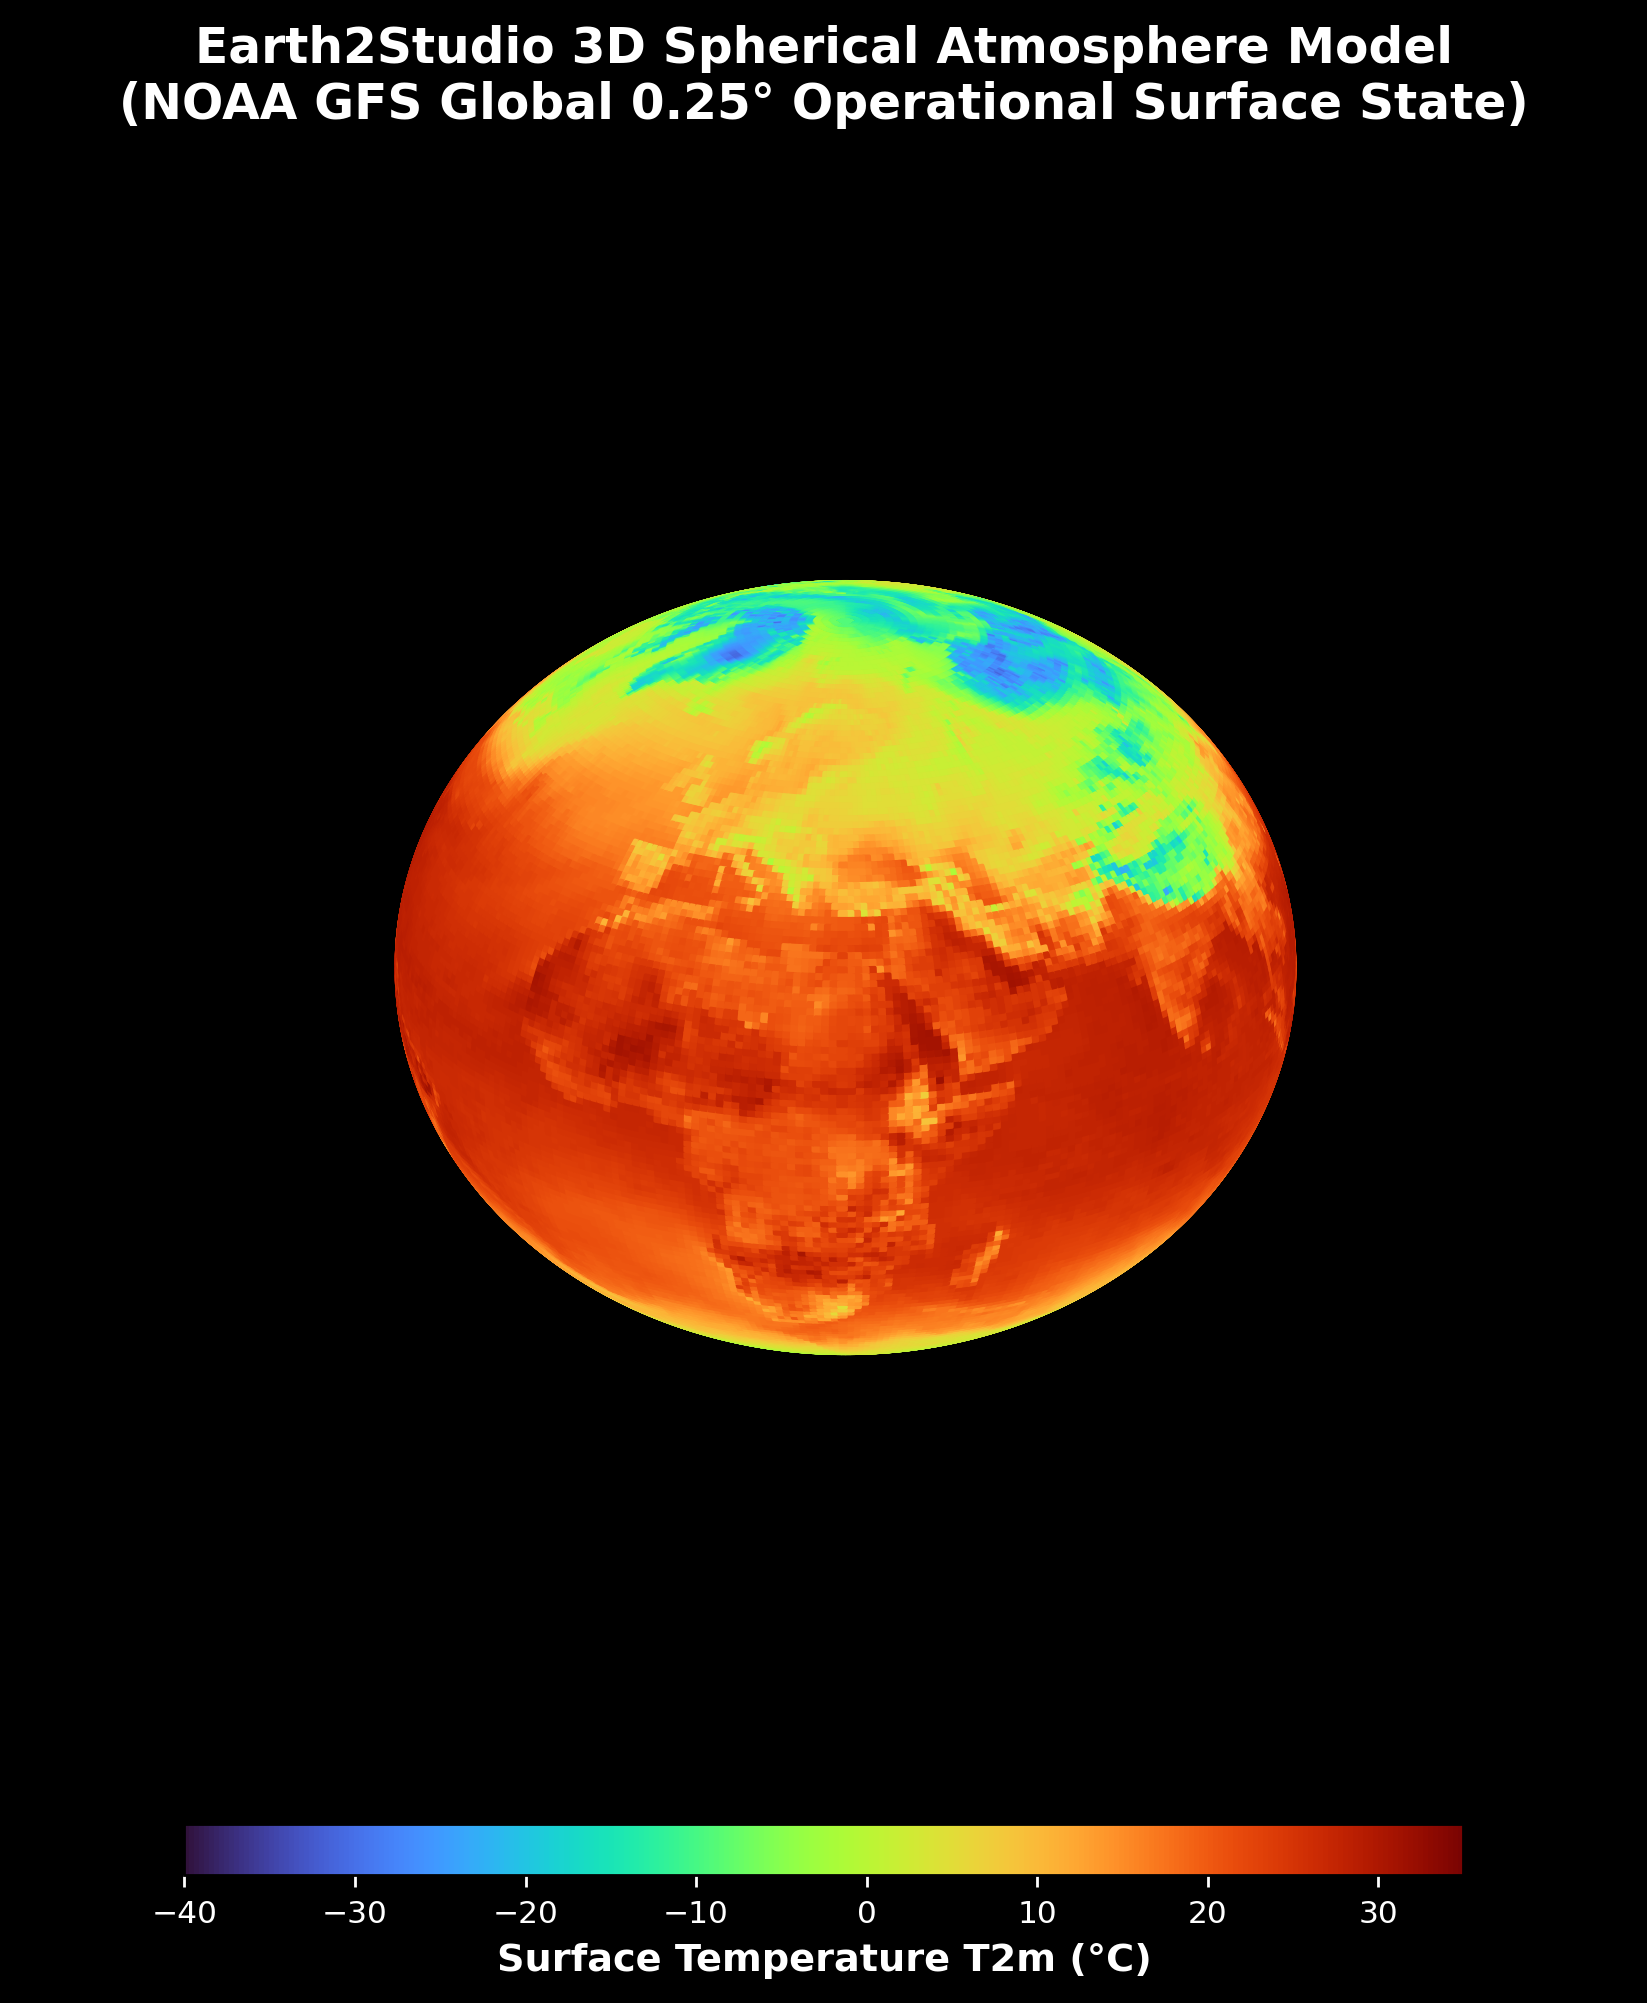
\includegraphics[width=\linewidth,height=1.75in,keepaspectratio]{earth_3d_spherical_model.png}\\[2pt]
    {\scriptsize\textit{Figure: Zero-dependency Three.js 3D Spherical Twin rendering 16K/131K LOD tiles and real-time streamlines at 60 FPS on 248 MB VRAM.}}

    \vspace{2pt}

    \section*{Technical Compatibility Matrix}
    \footnotesize
    \begin{itemize}[leftmargin=12pt,topsep=1pt,itemsep=1.5pt,parsep=0pt]
        \item \textbf{WebGL \& Graphics:} Three.js, WebGL 2.0, GLSL custom shaders, \texttt{ImageBitmapLoader}, frustum culling, dynamic LOD octants.
        \item \textbf{Spatial Standards:} OGC STAC v1.0.0, Cloud-Optimized GeoTIFF (COG), GeoJSON, EPSG:4326/WGS84, XYZ tile pyramids.
        \item \textbf{Frontend Architecture:} Modern vanilla ES6+ (zero framework bloat), responsive CSS, Chrome DevTools Protocol (CDP) automated testing.
        \item \textbf{Backend & Data Integration:} Python data preparation, GDAL/Rasterio, Vercel Edge deployment, WebSocket/REST APIs.
    \end{itemize}

    \section*{Direct Value to Planet Labs}
    \footnotesize
    \begin{tcolorbox}[colframe=planetteal,colback=white,boxrule=0.6pt,top=4pt,bottom=4pt]
    \textbf{Immediate Operational Impact:}
    \begin{itemize}[leftmargin=10pt,topsep=0pt,itemsep=1pt]
        \item Proven ability to build high-performance 3D geospatial web applications that run smoothly on consumer laptops and smartphones.
        \item Hands-on expertise in satellite image tiling, multi-resolution LOD rendering, and spatial metadata visualization.
        \item Production rigor backed by automated headless browser testing, CI/CD, and clean zero-dependency codebases.
    \end{itemize}
    \end{tcolorbox}
\end{minipage}

\vspace{-2pt}

% FOOTER CALL TO ACTION
\begin{tcolorbox}[colframe=planetblue,colback=planetblue,coltext=white,boxrule=0pt,top=4pt,bottom=4pt]
\centering\footnotesize
\textbf{Explore the Interactive Demo:} \href{https://earth2-sar-insar.vercel.app#preset=clean_globe&stage=v3}{\texttt{earth2-sar-insar.vercel.app\#preset=clean\_globe}} $\,\cdot\,$ 
\textbf{Contact Zhane Daye:} \texttt{zhanedaye@umattr.ca} $\,\cdot\,$ Available for technical review \& interviews.
\end{tcolorbox}

\end{document}
